%%%%%%%%%%%%%%%%%%%%%%%%%%%%%%%%%%%%%%%%%%%%%%%%%%%%%%%%%%%%%%%%%%%%%%%%%%
%% Review Volume (last updated on 20-4-2015)                            %%
%% Trim Size: 9in x 6in                                                 %%
%% Text Area: 7.35in (include runningheads) x 4.5in                     %%
%% Main Text: 10 on 13pt                                                %%
%% For support: Yolande Koh, <ykoh@wspc.com.sg>                         %%
%%              D. Rajesh Babu, <rajesh@wspc.com.sg>                    %%
%%%%%%%%%%%%%%%%%%%%%%%%%%%%%%%%%%%%%%%%%%%%%%%%%%%%%%%%%%%%%%%%%%%%%%%%%%
%%
%\documentclass[wsdraft]{ws-rv9x6} % to draw border line around text area
\documentclass{ws-rv9x6}
\usepackage{subfigure}   % required only when side-by-side / subfigures are used
\usepackage{ws-rv-thm}   % comment this line when `amsthm / theorem / ntheorem` package is used
\usepackage[square]{ws-rv-van}   % numbered citation & references (default)
%\usepackage{ws-index}   % to produce multiple indexes
\makeindex
%\newindex{aindx}{adx}{and}{Author Index}       %author index
%\renewindex{default}{idx}{ind}{Subject Index}  %subject index

\begin{document}

\chapter[Ancestral Reconstruction of Bat Echolocation Calls]{Phylogenetic Gaussian Processes for the Ancestral Reconstruction of Bat Echolocation Calls}\label{ra_ch1}

\author[J.P. Meagher \textit{et al.}]{J.P. Meagher\footnote{J.P Meagher would like to thank the EPSRC for funding this work, and also acknowledge the support of the Alan Turing Institute and Gaelic Players Association.}, T. Damoulas\footnote{The University of Warwick and The Alan Turing Institute}, K.E. Jones\footnote{Centre for Biodiversity and Environment Research, University College London}, and M. Girolami\footnote{Imperial College London and The Alan Turing Institute}\\}
%\index[aindx]{Author, F.} % or \aindx{Author, F.}
%\index[aindx]{Author, S.} % or \aindx{Author, S.}

\address{Department of Statistics,\\ The University of Warwick.\\
	J.Meagher@Warwick.ac.uk}

\begin{abstract}
The reconstruction of ancestral echolocation calls is an important part of understanding the evolutionary history of bats. General techniques for the ancestral reconstruction of function-valued traits have recently been proposed. A full implementation of phylogenetic Gaussian processes for the ancestral reconstruction of function-valued traits representing bat echolocation calls is presented here. A phylogenetic signal was found in the data and ancestral reconstruction performed. This promising preliminary analysis paves the way for more realistic models for the evolution of echolocation in bats.
\end{abstract}
%\markright{Customized Running Head for Odd Page} % default is Chapter Title.
\body

%\tableofcontents
\section{Introduction}
\label{sec:intro}
The emerging field of Data Science is driven by research which lies at the nexus of Statistics and Computer Science. Bioacoustics is one such area generating vast quantities of data, often through citizen science initiatives \cite{pettorelli2013indicator}. Bioacoustic techniques for biodiversity monitoring \cite{stathopoulos2017bat} \cite{damoulas2010bayesian} have the potential to make real policy impacts, particularly with regard to sustainable economic development and nature conservation.

Bats (order \textit{Chiroptera}) have been identified as ideal bioindicators for monitoring climate change and habitat quality \cite{jones2009carpe}, and are of particular interest for monitoring biodiversity acoustically. Typically, a bat broadcasts information about itself in an ultrasonic echolocation call \cite{griffin1944echolocation}. The development of automatic acoustic monitoring algorithms \cite{stathopoulos2017bat} \cite{walters2012continental} means that large scale, non-invasive monitoring of bats is becoming possible.   

Monitoring bat populations provides useful information, but an understanding of the evolutionary history is required to identify the cause and effect of any changes observed. The echolocation call structure, which reflects a bats diet and habitat \cite{aldridge1987morphology}, is a key aspect of this evolutionary history. Reconstructing ancestral traits \cite{joy2016ancestral} relies on a statistical comparative analysis incorporating extant species and fossil records \cite{felsenstein2004inferring}. However, the fossil record is of limited use in inferring ancestral echolocation calls in bats. Therefore, statistical data science techniques may shed some light on this topic.

Previous studies of bat echolocation calls for both classification \cite{walters2012continental} and ancestral reconstruction \cite{collen2012evolution} analysed features extracted from the call spectrogram. These call features relied upon domain knowledge to ensure they were sensibly selected and applied. More recently, general techniques for the classification of acoustic signals have been developed \cite{stathopoulos2014bat} \cite{damoulas2010bayesian}. General techniques for the ancestral reconstruction of function-valued traits have also been proposed \cite{group2012phylogenetic}. Jones \& Moriarty \cite{jones2013evolutionary} extend Gaussian Process Regression \cite{rasmussen2006gaussian} to model the evolution of function-valued traits \cite{meyer2005up} over a phylogeny, a method which was demonstrated for synthetic data by Hajipantelis \textit{et al.} \cite{hadjipantelis2013function}. This current research investigates these techniques in the context of the bat echolocation calls.

The structure of this paper is as follows, section \ref{sec:funrep} presents details on representing echolocation call recordings as function-valued traits. Section \ref{sec:pgp} develops the model for evolution given by a phylogenetic Gaussian Process. The results of the analysis of bat echolocation calls are then presented and discussed in sections \ref{sec:results} and \ref{sec:conc}.

\section{Echolocation Calls as Function-Valued Traits}
\label{sec:funrep}
A functional data object is generated when repeated measurements of some process are taken along a continuous scale, such as time \cite{ramsay2006functional}. 
These measurements can be thought of as representing points on a curve that varies gradually and continuously. In the context of phylogenetics, these functional data objects are function-valued traits \cite{meyer2005up}.

\begin{figure}
	\centering
	\subfigure[]{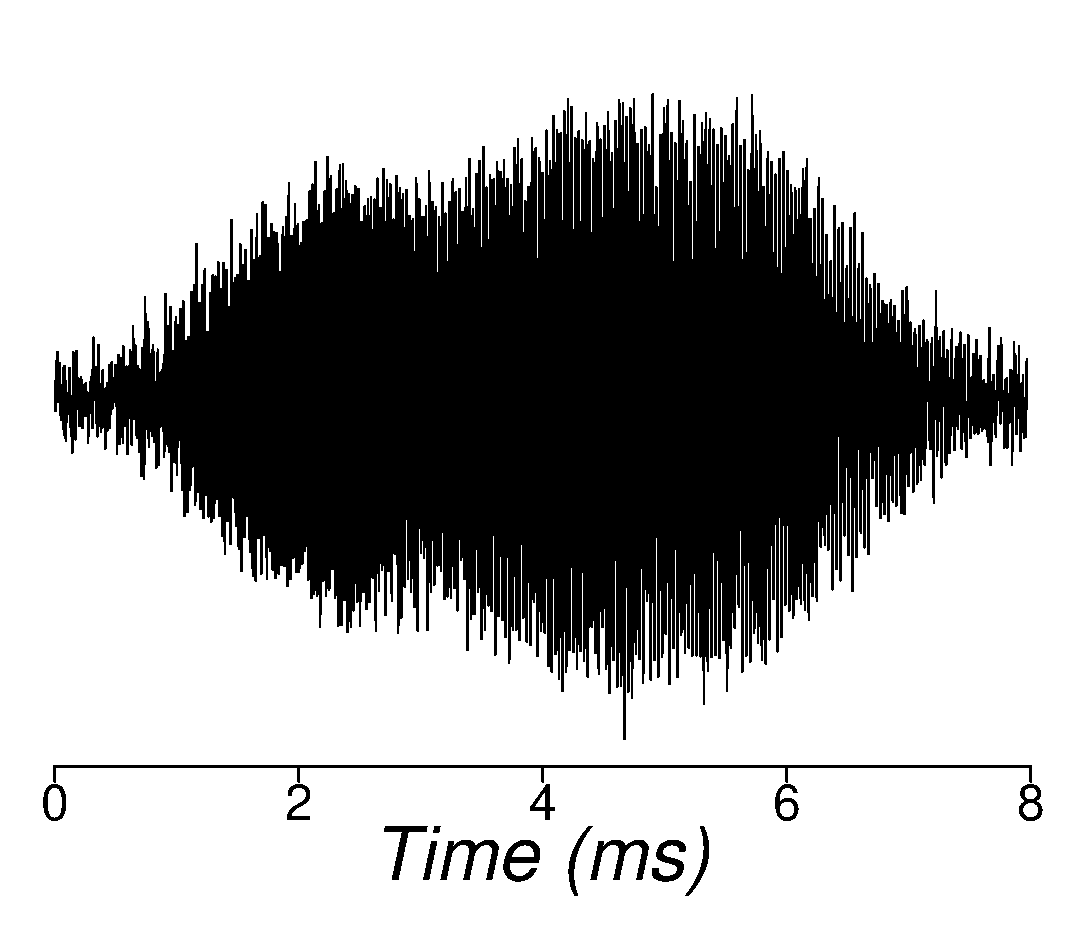
\includegraphics[width = 0.3\textwidth]{../Figures/callrec.eps} \label{fig:call}}
	\subfigure[]{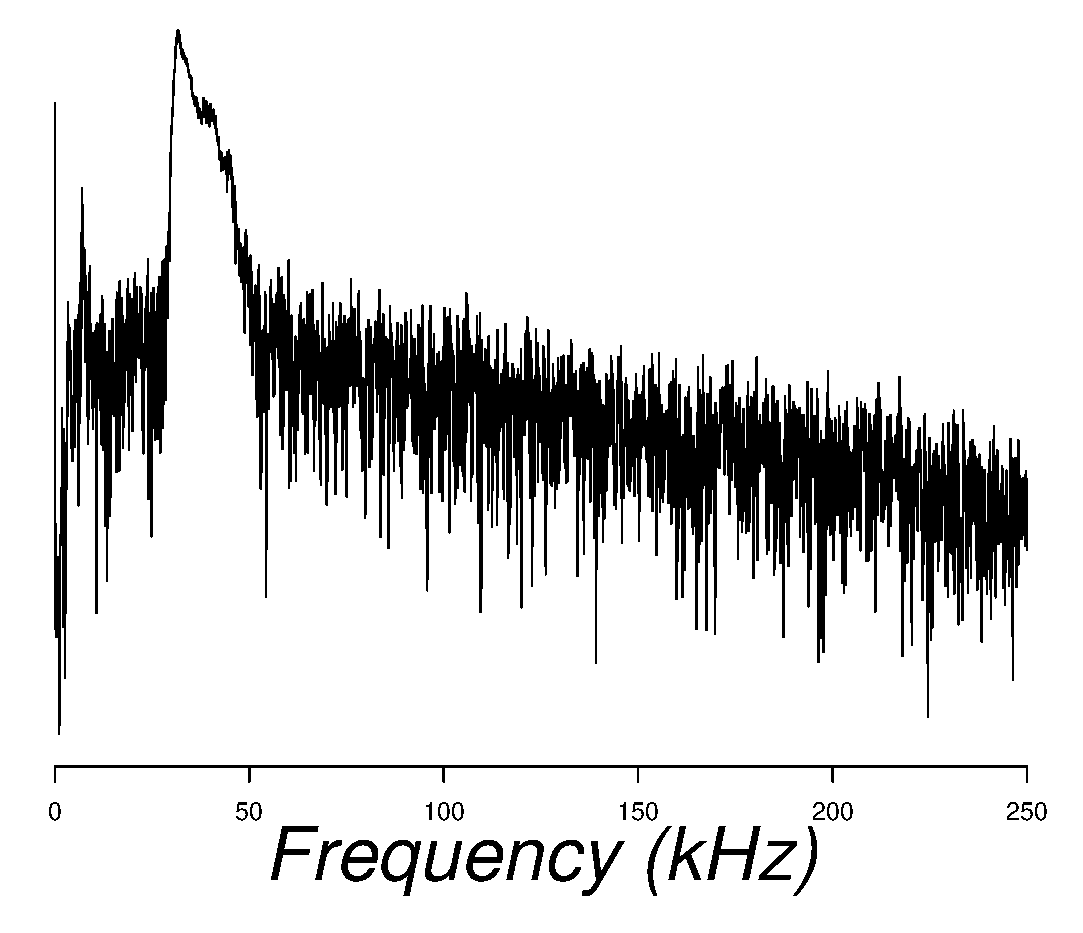
\includegraphics[width = 0.3\textwidth]{../Figures/esd.eps} \label{fig:esd}}
	\subfigure[]{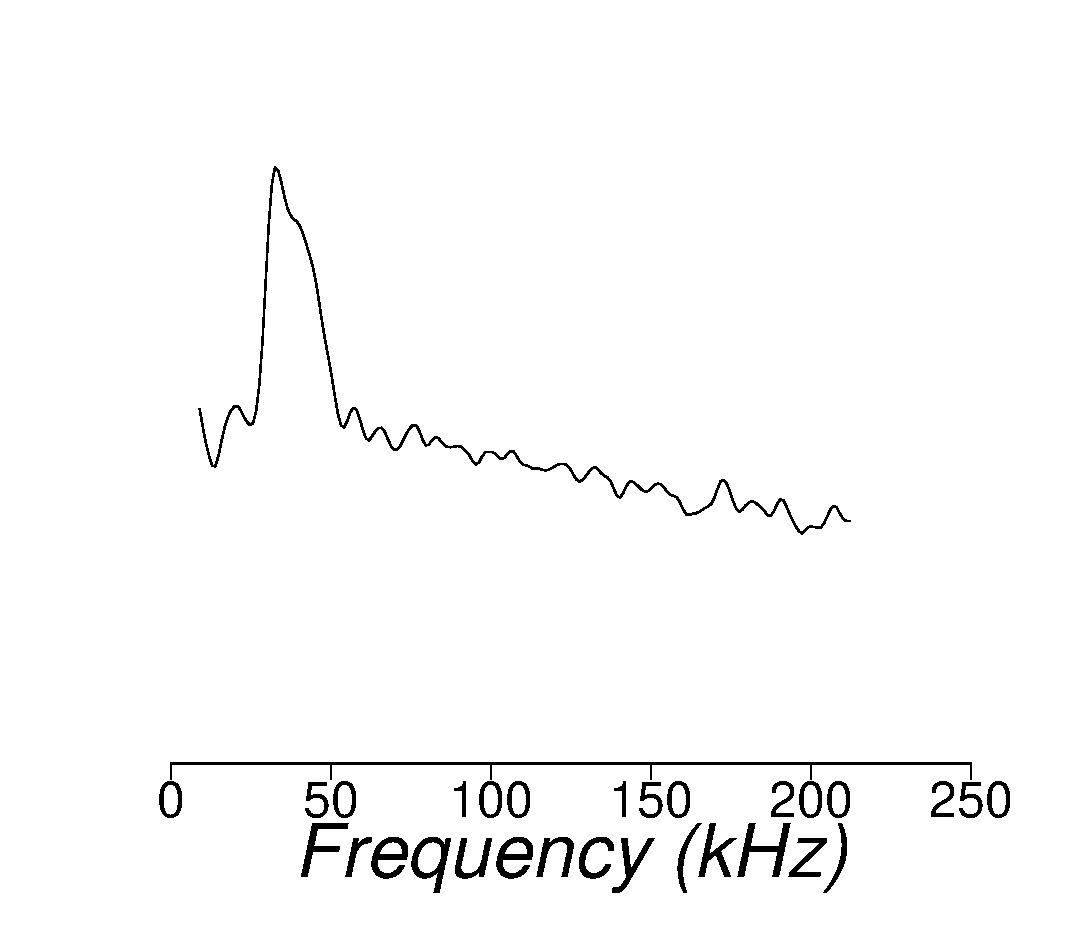
\includegraphics[width = 0.3\textwidth]{../Figures/funrep.eps} \label{fig:funrep}}
	\caption{A recording of a bat echolocation call (a) along with the log energy spectral density of the call (b) and the smooth functional representation of that spectral density restricted to the range \([9-212]\)kHz (c).}
\end{figure}

Given a phylogenetic tree \(\mathbf{T}\), representing the evolutionary relationships between the recorded bat species, we denote the \(m^{th}\) call recording of the \(l^{th}\) individual bat of the species observed at point \(\mathbf{t} \in \mathbf{T}\) by \(\{\hat{x}_{lm}^{\mathbf{t}}(n)\}_{n=0}^{N_{lm}^{\mathbf{t}} - 1}\). 
Thus, \(\{\hat{x}_{lm}^{\mathbf{t}}(n)\}\) is a series of discrete measurements of the function \(x_{lm}^{\mathbf{t}}(\cdot)\), observed at the time points given by \(\frac{n}{f_S}\), where \(f_S\) is the sampling rate, in samples per second (Hz), of the recording. Assume then that \(x_{lm}^{\mathbf{t}}(\cdot) = x_{l}^{\mathbf{t}}(\cdot) + z_{lm}^{\mathbf{t}}(\cdot)\), where \(x_{l}^{\mathbf{t}}(\cdot)\) is the representative call function for the \(l^{th}\) individual and \(z_{lm}^{\mathbf{t}}(\cdot)\) is the noise process for the \(m^{th}\) call. Further, assume that \(x_{l}^{\mathbf{t}}(\cdot) = x^{\mathbf{t}}(\cdot) + z_{l}^{\mathbf{t}}(\cdot)\) where \(x^{\mathbf{t}}(\cdot)\) is the representative call function for the bat species at \({\mathbf{t}}\) and \(z_{l}^{\mathbf{t}}(\cdot)\) is the noise process for the \(l^{th}\) individual. It is the phylogenetic relationship between the species level echolocation call functions that we are interested in modelling.

The call recordings themselves are functional data objects, however modelling the phylogenetic relationships between \(\{x_{lm}^{\mathbf{t}}(t)\}\) and \(\{x_{l'm'}^{{\mathbf{t}}'}(t)\}\) directly implies that the processes are comparable at time \(t\). 
This is not the case for acoustic signals, a phenomenon which is often addressed by dynamic time warping \cite{berndt1994using}. Another approach to this issue is to consider an alternative functional representation of the signal. 

The Fourier transform of \(x_{lm}^{\mathbf{t}}(\cdot)\) is given by
\[
X_{lm}^{\mathbf{t}}(f) = \int_{-\infty}^{\infty} x_{lm}^{\mathbf{t}}(t) e^{-i 2\pi f t} dt.
\label{eqn:dft}
\]
The energy spectral density of \(x_{lm}^{\mathbf{t}}(\cdot)\) is the squared magnitude of the Fourier transform and the log energy spectral density is given by
\[
\mathcal{E}_{lm}^{\mathbf{t}}(\cdot) = 10 \log_{10} \left( |X_{lm}^{\mathbf{t}}(\cdot)|^2 \right).
\]

Similarly to the call functions, \(\mathcal{E}_{lm}^{\mathbf{t}}(\cdot)\) is the log energy spectral density of the \(m^{th}\) call of the \(l^{th}\) individual from the species at \({\mathbf{t}}\) where \(\mathcal{E}_{lm}^{\mathbf{t}}(\cdot) = \mathcal{E}_{l}^{\mathbf{t}}(\cdot) + \mathcal{Z}_{lm}^{\mathbf{t}}(\cdot)\) and \(\mathcal{E}_{l}^{\mathbf{t}}(\cdot) = \mathcal{E}^{\mathbf{t}}(\cdot) + \mathcal{Z}_{l}^{\mathbf{t}}(\cdot)\) where \(\mathcal{Z}_{lm}^{\mathbf{t}}(\cdot)\) and \(\mathcal{Z}_{l}^{\mathbf{t}}(\cdot)\) are noise processes, each with an expected value of zero.  The log energy spectral density is a periodic function of frequency which describes the energy of a signal at each frequency on the interval \(F = [0, \frac{f_S}{2}]\).\cite{antoniou2006digital}

The discrete Fourier Transform \cite{antoniou2006digital}
of \(\{\hat{x}_{lm}^{\mathbf{t}}(n)\}\) provides an estimate for the log energy spectral density, the positive frequencies of which are denoted \(\{\mathcal{E}_{lm}^{\mathbf{t}}(k) : k = 0, \dots, \frac{ N_{lm}^{\mathbf{t}}}{2} + 1\}\). Smoothing splines \cite{friedman2001elements} are applied to this series to obtain \(\hat{\mathcal{E}}_{lm}^{\mathbf{t}}(\cdot)\), a smooth function estimating \(\mathcal{E}_{lm}^{\mathbf{t}}(\cdot)\).

We now have a functional representation of each bats echolocation call where the pairs of observations \(\{f, \hat{\mathcal{E}}_{lm}^{\mathbf{t}}(f)\}\) and \(\{f, \hat{\mathcal{E}}_{l'm'}^{{\mathbf{t}}'}(f)\}\) are directly comparable. These function-valued traits can now be modelled for evolutionary inference.

\section{Phylogenetic Gaussian Processes}
\label{sec:pgp}
A Gaussian process places a prior distribution over functions, \(f(x) \sim \mathcal{GP}(m(x), k (x, x'))\), where \(x \in \mathbf{R}^P\) is some input variable, the mean function \(m(x) = \mathbf{E}[f(x)]\), and the covariance function \(k(x, x') = \mathrm{cov}(f(x), f(x') )\). Given observations \(\mathbf{y}\) at locations \(\{x_n\}_{n=1}^N\), Gaussian noise, and kernel hyperparameters \(\theta\), a posterior predictive distribution over functions can be inferred analytically. See Rasmussen \& Williams \cite{rasmussen2006gaussian} for an in depth treatment.   

Jones \& Moriarty \cite{jones2013evolutionary} extend GPs for the inference of function-valued traits over a phylogeny. Consider \(\mathcal{E}^{\mathbf{t}}(\cdot)\), a functional representation of the echolocation call of the species observed at the point \(\mathbf{t}\) on the phylogenetic tree \(\mathbf{T}\) with respect to frequency. Modelling this as GP function, where \(\mathcal{E}^{\mathbf{t}}(f)\) corresponds to a point \((f, \mathbf{t})\) on the frequency-phylogeny \(F \times \mathbf{T}\), requires that a suitable phylogenetic covariance function, \(\Sigma_{\mathbf{T}}\left((f,\mathbf{t}), (f',\mathbf{t}')\right)\), is defined.

\begin{figure}[h]
	\subfigure[]{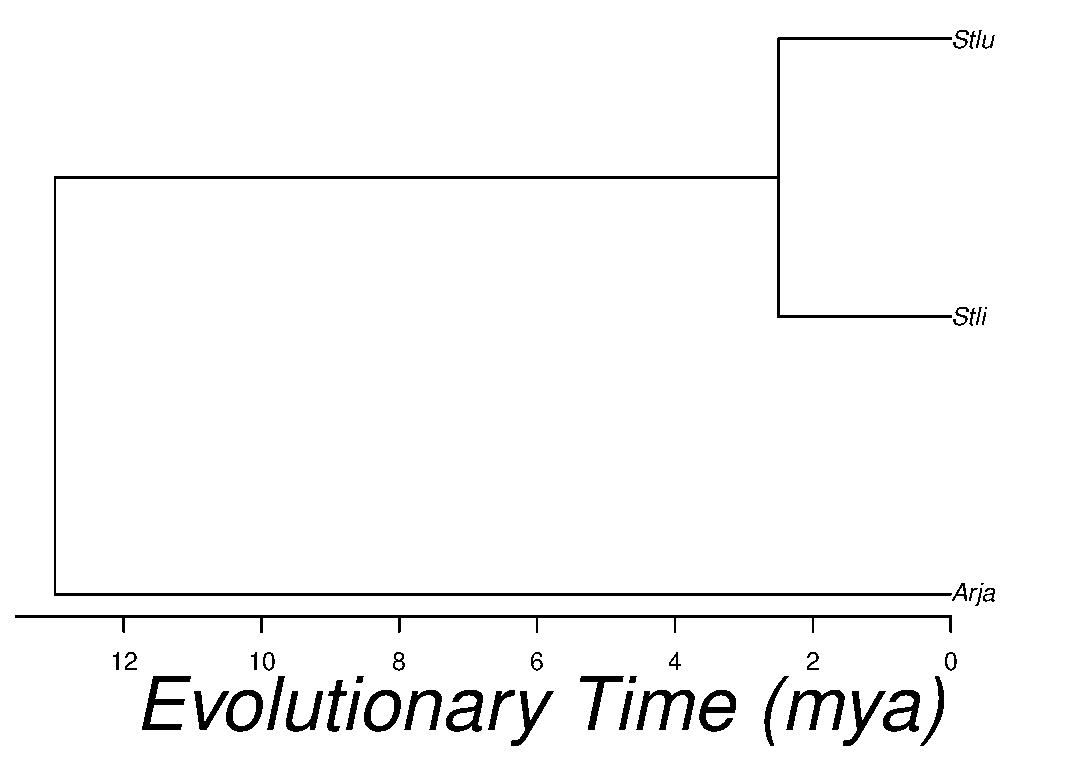
\includegraphics[width = 0.45\textwidth]{../Figures/tree3} }
	\subfigure[]{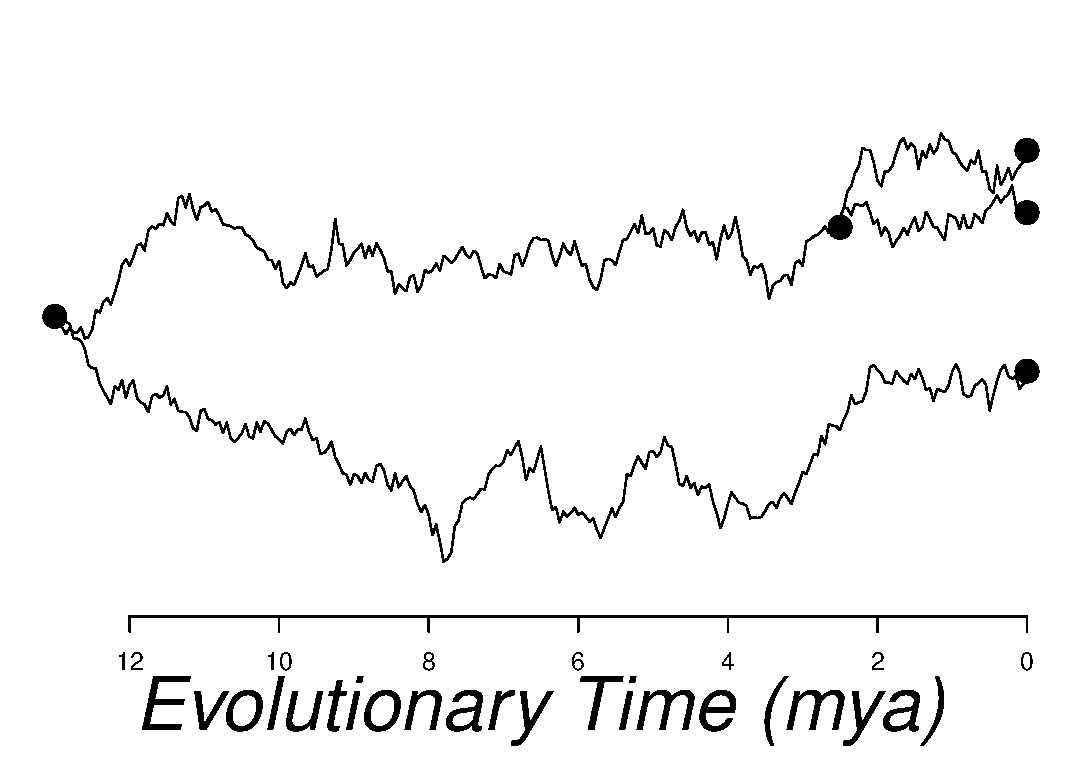
\includegraphics[width = 0.45\textwidth]{../Figures/unipgp} }
	\caption{A sub tree from the full phylogeny \(\mathbf{T}\) (a) and a simulated univariate phylogenetic OU GP over that sub tree (b).}
	\label{fig:subtree}
\end{figure}

Deriving a tractable form of the phylogenetic covariance function requires some simplifying assumptions. Firstly, it is assumed that conditional on their common ancestors in the phylogenetic tree \(\mathbf{T}\), any two traits are statistically independent. 

The second assumption is that the statistical relationship between a trait and any of it's descendants in \(\mathbf{T}\) is independent of the topology of \(\mathbf{T}\). That is to say that the underlying process driving evolutionary changes is identical along all individual branches of the tree. We call this underlying process along each branch the marginal process. The marginal process depends on the date of \(\mathbf{t}\), the distance between \(\mathbf{t}\) and the root of \(\mathbf{T}\), denoted \(t\). 

Finally, it is assumed that the covariance function of the marginal process is separable over evolutionary time and the function-valued trait space. Thus, by defining the frequency only covariance function \(K(f,f')\) and the time only covariance function \(k(t,t')\) the covariance function of the marginal process is \(\Sigma\left((f,t), (f',t')\right) = K(f, f') k(t,t')\).

Under these conditions the phylogenetic covariance function is also separable and so
\begin{equation}
\Sigma_{\mathbf{T}}\left((f,\mathbf{t}), (f',\mathbf{t}')\right) = K(f, f') k_{\mathbf{T}}(\mathbf{t},\mathbf{t}').
\label{eqn:phy}
\end{equation}

For a phylogenetic Gaussian Process \(Y\) with covariance function given by (\ref{eqn:phy}), when \(K\) is a degenerate Mercer kernel, there exists a set of \(n\) deterministic basis functions \(\phi_i: F \to \mathbf{R}\) and univariate GPs \(X_i\) for \(i = 1,\dots, n\) such that 
\[
g(f, \mathbf{t}) = \sum_{i = 1}^{n} \phi_i(f) X_i(\mathbf{t})
\] 
has the same distribution as \(Y\). The full phylogenetic covariance function of this phylogenetic GP is
\[
\Sigma_{\mathbf{T}}((f, \mathbf{t}), (f', \mathbf{t}')) = \sum_{i = 1}^{n}  k_{\mathbf{T}}^i(\mathbf{t}, \mathbf{t}') \phi_i(f) \phi_i(f'),
\]
where \(\int \phi_i(f) \phi_j(f) df = \delta_{ij}\), \(\delta\) being the Kronecker delta, and so the phylogenetic covariance function depends only on \(\mathbf{t}, \mathbf{t}' \in \mathbf{T}\). 

Thus, given function-valued traits observed at \(\mathbf{f} \times \mathcal{t}\) on the frequency-phylogeny, where \(\mathbf{f} = [f_1, \dots, f_q]^{\mathsf{T}}\) and \(\mathcal{t} = [\mathbf{t}_1, \dots, \mathbf{t}_Q]^{\mathbf{T}}\), an appropriate set of basis functions \(\phi_{F} = [\phi^{F}_1(\mathbf{f}), \dots, \phi^{F}_n(\mathbf{f})]\) for the traits \(\mathcal{E} = [\mathcal{E}^{\mathbf{t}}(\mathbf{f}), \dots, \mathcal{E}^{\mathbf{t}'}(\mathbf{f})]\), and Gaussian Processes, \(X_{\mathbf{T}} = [X_1^{\mathbf{T}}(\mathcal{t}), \dots\ X_n^{\mathbf{T}}(\mathcal{t})]\), the set of observations of the echolocation function-valued trait are then 
\begin{equation}
\mathcal{E} = X_{\mathbf{T}} \phi_F^{\mathsf{T}}.
\label{eqn:inv}
\end{equation}

The problem of obtaining estimators \(\hat{\phi}_F\) and \(\hat{X}_{\mathbf{T}}\) is dealt with by Hajipantelis \textit{et al.} \cite{hadjipantelis2013function}. \(\hat{\phi}_F\) is obtained by Independent Components Analysis, as described by Blaschke \& Wiscott \cite{blaschke2004cubica} after using a resampling procedure to obtain stable principal components for the observed traits. Given \(\hat{\phi}_F\), the estimated matrix of mixing coefficients is \(\hat{X}_{\mathbf{T}} = \mathcal{E} (\hat{\phi}_F^{\mathsf{T}})^{-1}\). 

\begin{figure}[h]
	\centering
	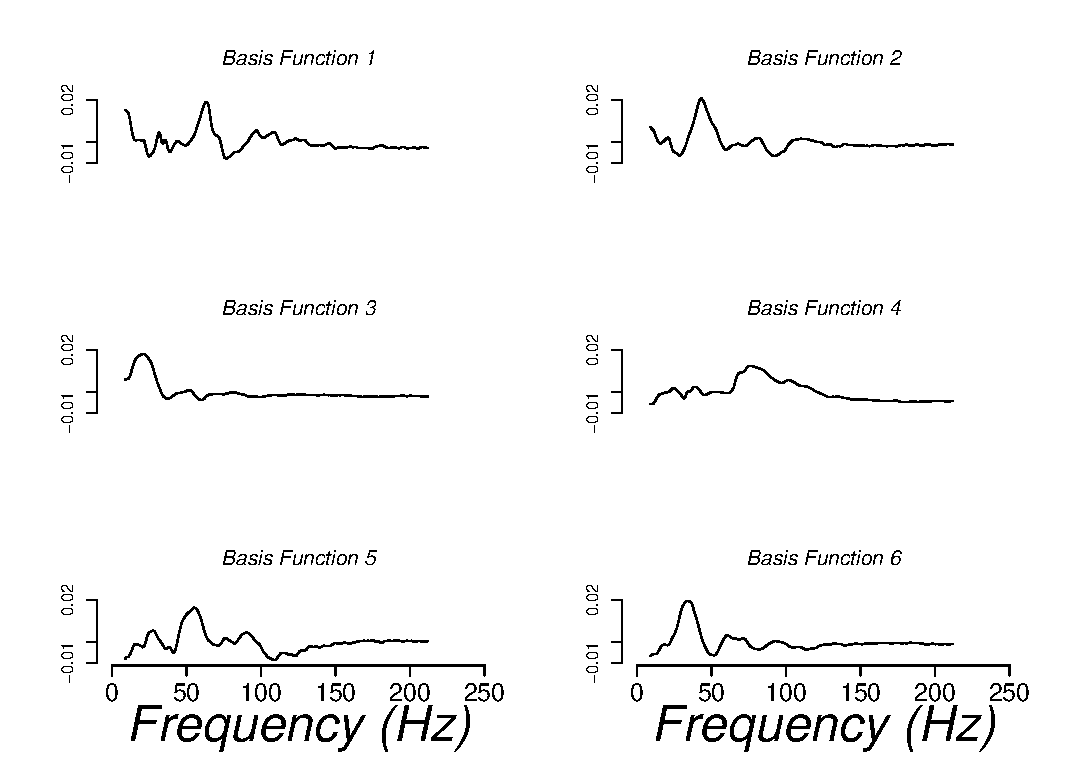
\includegraphics[width = 0.9\textwidth]{../Figures/basis.eps}
	\caption{Set of independently evolving basis functions identified for bat echolocation calls. }
\end{figure}

Each column of \(X_{\mathbf{T}}\) is an independent, univariate, phylogenetic GP, \(X_i^{\mathbf{T}}(\mathcal{t})\), modelled here with phylogenetic Ornstein-Uhlenbeck (OU) process kernel.

The phylogenetic OU process is defined by the kernel
\begin{equation}
k_{\mathbf{T}}^i(\mathbf{t}, \mathbf{t}') = (\sigma_p^i)^2 \exp \left( \frac{-d_{\mathbf{T}}(\mathbf{t}, \mathbf{t}')}{\ell^i} \right) + (\sigma_n^i)^2 \delta_{\mathbf{t}, \mathbf{t}'}
\label{eqn:oukernel}
\end{equation}

where \(\delta\) is the Kronecker delta, \(d_{\mathbf{T}}(\mathbf{t}, \mathbf{t}')\) is the distance along \(\mathbf{T}\) between \(\mathbf{t}\) and \(\mathbf{t}' \in \mathbf{T}\), and \(\mathbf{\theta}^i = [\sigma_p^i, \ell^i, \sigma_n^i]^{\mathsf{T}}\) is the vector of hyperparameters for \(X_i^{\mathbf{T}}(\cdot)\). The phylogenetic covariance matrix for \(X_i^{\mathbf{T}}(\mathcal{t})\) is denoted \(\Sigma_{\mathbf{T}}^i(\mathcal{t}, \mathcal{t})\) and the marginal likelihood of the observed data given \(\theta\) is
\begin{equation}
\log(p(\mathcal{E} | \theta)) \propto -\frac{1}{2} \sum_{i = 1}^{n} \left( X_i(\mathcal{t})^{\mathsf{T}} \Sigma_{\mathbf{T}}^i(\mathcal{t}, \mathcal{t})^{-1}  X_i(\mathcal{t}) + \log |\Sigma_{\mathbf{T}}^i(\mathcal{t}, \mathcal{t})|    \right)
\label{eqn:t2mle}
\end{equation}
and so \(\theta\) can be estimated by type II maximum likelihood estimation.

Ancestral Reconstruction of the function valued trait for the species at \(\mathbf{t}^*\) then amounts to inferring the posterior predictive distribution \(p(\mathcal{E}^{\mathbf{t}^*} (\cdot) | \mathcal{E}) \sim \mathcal{N}(A, B)\) where 
\begin{equation}
A = \sum_{i=1}^{n} \left( \Sigma_{\mathbf{T}}^i(\mathbf{t}^*, \mathcal{t}) \left( \Sigma_{\mathbf{T}}^i(\mathcal{t}, \mathcal{t})
\right)^{-1} X_i^{\mathcal{E}} (\mathcal{t}) \phi_i(\cdot) \right)
\label{eqn:postmean}
\end{equation}
\begin{equation}
B = \sum_{i=1}^{n}\left( \Sigma_{\mathbf{T}}^i(\mathbf{t}^*, \mathbf{t}^*) -  \Sigma_{\mathbf{T}}^i(\mathbf{t}^*, \mathcal{t}) \left( \Sigma_{\mathbf{T}}^i(\mathcal{t}, \mathcal{t})
\right)^{-1} \Sigma_{\mathbf{T}}^i(\mathbf{t}^*, \mathcal{t})^{\mathsf{T}} \right) \phi_i (\cdot)
\label{eqn:postvar}
\end{equation}

We note that the elements of \(\theta\) each have intuitive interpretations. The total variation of observed points is \(\sigma_p + \sigma_n\), where \(\sigma_p\) is the phylogenetic noise, and \(\sigma_n\) is the non-phylogenetic noise. \(\sigma_p\) is the variation depending on the evolutionary time between any \(\mathbf{t}, \mathbf{t}' \in \mathbf{T}\), while \(\sigma_n\) accounts for variation that does not depend on the phylogeny. The length-scale parameter, \(\ell\), indicates the strength of the correlation between points on \(\mathbf{T}\), where large values of \(\ell\) indicate a correlation that decays slowly as \(d_{\mathbf{T}}(\mathbf{t}, \mathbf{t}')\) increases. 

\section{Results}
\label{sec:results}
\subsection{Data Description}

Post processed echolocation call data accompanying Stathopoulos \textit{et al.} \cite{stathopoulos2017bat} was used in this analysis. Live bats were caught, identified, and recorded at a sampling frequency of 500 kHz. 
In total the dataset consists of 22 species from five families, 449 individual bats and 1816 individual echolocation call recordings. The distribution of these call recordings across species is summarised in Table \ref{tab::dataset}.

Collen's \cite{collen2012evolution} Bat super-tree provided the phylogenetic tree of the recorded bat species, \(\mathbf{T}\). 

\begin{table}[ht]
	\tbl{Echolocation Call Dataset}
	{\begin{tabular}{@{}lccc@{}} \toprule
			Species & Key & Individuals & Calls \\ \colrule
			Family: Emballonuridae &&& \\
			1 \textit{Balantiopteryx plicata} & Bapl & 16 & 100 \\
			\colrule
			Family: Molossidae &&& \\
			2 \textit{Nyctinomops femorosaccus} & Nyfe & 16 & 100 \\
			3 \textit{Tadarida brasiliensis} & Tabr & 49 & 100  \\
			\colrule
			Family: Vespertilionidae &&& \\
			4 \textit{Antrozous pallidus} & Anpa & 58 & 100 \\
			5 \textit{Eptesicus fuscus} & Epfu & 74 & 100 \\
			6 \textit{Idionycteris phyllotis} & Idph & 6 & 100 \\
			7 \textit{Lasiurus blossevillii} & Labl & 10 & 90 \\
			8 \textit{Lasiurus cinereus} & Laci & 5 & 42 \\
			9 \textit{Lasiurus xanthinus} & Laxa & 8 & 100 \\
			10 \textit{Myotis volans} & Myvo & 8 & 100 \\
			11 \textit{Myotis yumanensis} & Myyu & 5 & 89 \\
			12 \textit{Pipistrellus hesperus} & Pihe & 85 & 100 \\
			\colrule
			Family: Mormoopidae &&& \\
			13 \textit{Mormoops megalophylla} & Mome & 10 & 100 \\
			14 \textit{Pteronotus davyi} & Ptda & 8 & 100 \\
			15 \textit{Pteronotus parnellii} & Ptpa & 23 & 100 \\
			16 \textit{Pteronotus personatus} & Ptpe & 7 & 51 \\
			\colrule
			Family: Phyllostomidae &&& \\
			17 \textit{Artibeus jamaicensis} & Arja & 11 & 82 \\
			18 \textit{Desmodus rotundus} & Dero & 6 & 38 \\
			19 \textit{Leptonycteris yerbabuenae} & Leye & 26 & 100 \\
			20 \textit{Macrotus californicus} & Maca & 6 & 53 \\
			21 \textit{Sturnira ludovici} & Stlu & 8 & 51 \\
			22 \textit{Sturnira lilium} & Stli & 4 & 20 \\
			\botrule
		\end{tabular}
	}
	\label{tab::dataset}
\end{table}

\subsection{Hyperparameter Estimation and Ancestral Trait Reconstruction with Phylogenetic Gaussian Processes}

We are interested in modelling the evolution of \(\mathcal{E}^{\mathbf{t}}(\cdot)\), the function valued trait representing \(x_{lm}^{\mathbf{t}}(\cdot)\), with a phylogenetic GP. However, only 22 species of bat are represented in \(\mathbf{T}\). The relatively small size of this dataset presents challenges for the estimation of the kernel hyperparameters in (\ref{eqn:oukernel}). A short simulation study was performed to investigate the the accuracy of estimated hyperparameters for a phylogenetic GP over \(\mathbf{T}\).

We are not limited to a single observation at any given \(\mathbf{t}\). By repeatedly sampling at each observed \(\mathbf{t}\), larger samples can be obtained, improving the quality of the estimators \(\hat{\theta}\). With this in mind, 1000 independent, univariate phylogenetic GPs were simulated for each of \(n = \{1,2,4,8\}\) according to the kernel (\ref{eqn:oukernel}) with \(\theta = [1,50,1]^{\mathsf{T}}\), where \(n\) is the number of samples generated at each leaf node. The likelihood of each of these samples (\ref{eqn:t2mle}) is then maximised to give a type II maximum likelihood estimator \(\hat{\theta}\) and the results summarised in Table \ref{tab::ind_simulation}. This simulation study indicates that at least \(n = 4\) observations are needed at each leaf node to provide stable estimators \(\hat{\theta}\).

\begin{table}[ht]
	\tbl{Summary of \(\hat{\theta}\) for 1000 simulations of independent OU processes with \(\theta = [1,50,1]^{\mathsf{T}}\) reporting: sample mean (standard error) }
	{
		\begin{tabular}{@{}cccc@{}} \toprule
			\(n\)  & \(\hat{\sigma}_p \) & \(\hat{\ell}\) & \(\hat{\sigma}_n\) \\
			\colrule
			1 & 1.09 (0.47) & \(10^{14}\) (\(10^{15}\)) & 0.57 (0.54) \\
			2 & 0.97 (0.29) & \(10^{13}\) (\(10^{14}\)) & 0.99 (0.15) \\
			4 & 0.97 (0.25) & 63.66 (136.96) & 1.00 (0.09) \\
			8 & 0.99 (0.24) & 56.21 ( 48.24) & 1.00 (0.06) \\			
			\botrule
		\end{tabular}
	}
	\label{tab::ind_simulation}
\end{table}

Given the modelling assumptions made in Section \ref{sec:funrep} an unbiased estimator for \(\mathcal{E}^{\mathbf{t}}(\cdot)\) is the sample mean given by 
\begin{equation}
\hat{\mathcal{E}}^{\mathbf{t}}~(\cdot) = \frac{1}{l_{\mathbf{t}}} \sum_{l = 1}^{l_{\mathbf{t}}} \frac{1}{m_l} \sum_{m = 1}^{m_l} \hat{\mathcal{E}}_{lm}^{\mathbf{t}}(\cdot)
\label{eqn:est}
\end{equation}
where \(m_l\) is the total number of recordings for the \(l^{th}\) individual and \(l_{\mathbf{t}}\) is the number of individuals recorded from the species at \(\mathbf{t} \in \mathbf{T}\). However, Table \ref{tab::ind_simulation} indicates that 22 samples is not enough to obtain a stable \(\hat{\theta}\) by type II maximum likelihood estimation. We implement a resampling procedure to leverage multiple estimates for each \(\mathcal{E}^{\mathbf{t}}(\cdot)\) from the dataset. This will produce a stable estimator, \(\hat{\theta}\).

A resampled estimator \(\hat{\mathcal{E}}_r^{\mathbf{t}}(\cdot)\) is obtained by sampling at random one call from \(n_r\) individuals of the species at \(\mathbf{t}\) and calculating the arithmetic mean of the sample, similarly to (\ref{eqn:est}). This can be repeated to create an arbitrary number of estimates for \(\mathcal{E}^{\mathbf{t}}\). Resampling across all the species in the dataset we create a resampled dataset \(\hat{\mathcal{E}}_r = [\hat{\mathcal{E}}_{r,1}^{\mathbf{t}_1}(\mathbf
f), \hat{\mathcal{E}}_{r,2}^{\mathbf{t}_1}(\mathbf
f), \dots, \hat{\mathcal{E}}_{r,1}^{\mathbf{t}_2}(\mathbf
f), \dots]\), where \(\mathbf{f}\) is the vector of frequencies over which \(\hat{\mathcal{E}}_{r}^{\mathbf{t}_2}(
\cdot)\) is sampled. The methods outlined in Section \ref{sec:pgp} can then be applied to each resampled \(\hat{\mathcal{E}}_r\)

Our analysis set \(n_r = 4\) and included 4 samples of \(\hat{\mathcal{E}}_r^{\mathbf{t}}(\mathbf{f})\) in each \(\hat{\mathcal{E}}_r\) for \(r = 1,\dots,1000\). This reflected the structure of the dataset, for which the minimum number of individuals per species was 4, and the results of the simulations study which showed that 4 observations per species provided reasonably stable estimates for \(\theta\). Note also that \(\mathbf{f} = [9,10, \dots, 212]^{\mathsf{T}}\), which reflects the spectrum of frequencies over which bats emit echolocation calls. \(\hat{\phi}_F\) was obtained by identifying the first six principal components, which accounted for approximately 85\% of the variation, in each  \(\hat{\mathcal{E}}_r\). By averaging over each sample, a single set of six stable, approximately orthogonal, basis functions were identified. These basis functions were then passed through Blaschke \& Wiscott's \cite{blaschke2004cubica} algorithm to produce a set of six independent basis functions for \(\mathcal{E}^\mathbf{t}(\cdot)\). Thus \(\hat{X}_r\), the matrix of mixing coefficients described by (\ref{eqn:inv}), the columns of which are modelled a phylogenetic OU processes, is obtained for each \(\hat{\mathcal{E}}_r\). \(\hat{\theta}_r\) is then the type II maximum likelihood estimator of (\ref{eqn:t2mle}) given \(\hat{\mathcal{E}}_r\). Table \ref{tab::bat_results} presents the results of the hyperparameter estimation procedure.

\begin{table}[ht]
	\tbl{Summary of \(\hat{\theta}_r\) over 1000 \(\hat{\mathcal{E}_r}\) samples reporting: sample mean (standard error)}
	{
		\begin{tabular}{@{}cccc@{}} \toprule
			Basis & \(\hat{\sigma}_p\) & \(\hat{\ell}\) & \(\hat{\sigma}_n\) \\
			\colrule
			1 & 2.30 (0.11) & 12.27 ( 4.18) & 1.18 (0.11) \\
			2 & 3.17 (0.11) & 27.63 ( 3.70) & 1.26 (0.13) \\
			3 & 4.05 (0.32) & 70.50 (20.31) & 1.19 (0.12) \\
			4 & 3.32 (0.17) & 22.86 ( 8.95) & 1.96 (0.19) \\
			5 & 3.00 (0.13) & 26.93 ( 2.85) & 1.21 (0.11) \\
			6 & 3.70 (0.14) & 12.82 ( 4.52) & 1.28 (0.15) \\
			\botrule
		\end{tabular}
	}
	\label{tab::bat_results}
\end{table}

Ancestral reconstruction by a phylogenetic GP involves obtaining the posterior predictive distribution of the trait at the ancestral node \(\mathbf{t}^* \in \mathbf{T}\) given by (\ref{eqn:postmean}) and (\ref{eqn:postvar}).

To perform ancestral trait reconstruction for \(\mathcal{E}^{\mathbf{t}^*}(\cdot)\) the species level traits are estimated by (\ref{eqn:est}) and and the model hyperparameters are set to be the mean values of \(\theta_r\) reported in Table \ref{tab::bat_results}.

\begin{figure}[h]
	\centering
	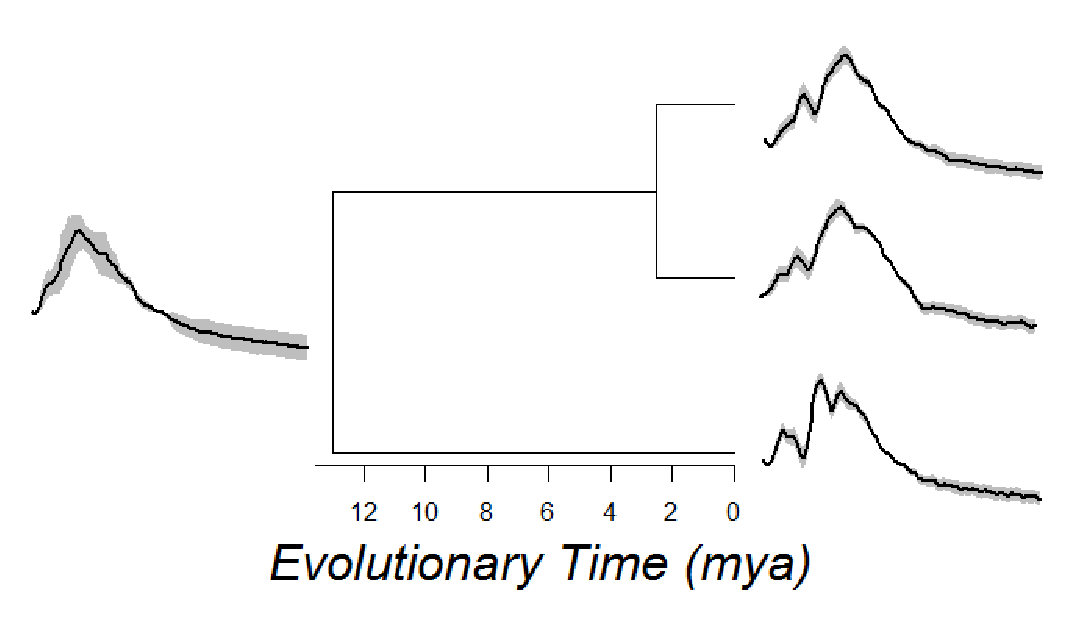
\includegraphics[width = 0.9\textwidth]{../Figures/ancrec.eps}
	\caption{Ancestral Reconstruction of the function valued trait representing the echolocation calls of the bat species included in the sub tree shown in Figure  \ref{fig:subtree} (a). Grey shaded region represents one standard deviation of variation around \(\hat{\mathcal{E}}^{\mathbf{t}}(\cdot)\).}
\end{figure}

\section{Conclusions and Further Work}
\label{sec:conc}
This preliminary analysis has developed a model for the evolution of echolocation in bats and identified a phylogenetic signal which allows the construction of a posterior predictive distribution for ancestral traits. The log energy spectral density has been identified as a trait representative of the echolocation call in bats. This trait, representing the energy intensity of the call across the frequency spectrum, is modelled as a series of independent components, combinations of energy intensities across the spectrum, each of which evolves according to a phylogenetic Ornstein-Uhlenbeck process. Estimating the hyperparameters governing these Ornstein-Uhlenbeck processes from observed traits provides an insight into the evolution of these traits. Each of the hyperparameters has an intuitive interpretation where \(\frac{\sigma_p}{\sigma_p + \sigma_n}\) indicates the proportion of variation in the sample accounted for by the phylogenetic distance between species, while \(\ell\) provides a measure of how quickly correlation along the phylogeny decays. We are working towards understanding what the results of this analysis could mean with respect to the evolution of echolocation in bats.

One particular limitation of the model is the representation of the echolocation call by a log energy spectral density. Echolocation calls have complex spectral and temporal structures, much of which is lost in the log energy spectral density representation. An alternative time-frequency representation, which preserves more of this structure, is the spectrogram. Modelling the evolution of bat echolocation calls with spectrograms, and implementing this model for a larger dataset of bat echolocation calls, is to be the subject of future research.

The interested reader can access the datasets and code used to produce these results through the R package 'sdsBAT' which is still under development and can be found at https://github.com/jpmeagher/sdsBAT.
\bibliographystyle{ws-rv-van}
\bibliography{../BatBiblio}

%\blankpage
%\printindex[aindx]                 % to print author index
%\printindex                         % to print subject index

\end{document} 